\section{Case Study II: Sugarscape}
\label{sec:sugarscape_concurrent}
The second case study is the Sugarscape model as introduced in Chapter \ref{sec:sugarscape}. In this case study we look into the potential for performance improvement in a model with much more complex agent behaviour and dramatically increased writes on the shared environment.

We implemented the \textit{Carrying Capacity} (p. 30) section of Chapter II of the Sugarscape book \cite{epstein_growing_1996}. In each step agents move to the cell with the highest sugar they see within their vision, harvest all of it from the environment, and consume sugar because of their metabolism. Sugar regrows in the environment over time. Only one agent can occupy a cell at a time. Agents don't age and cannot die from age. If agents run out of sugar due to their metabolism, they die from starvation and are removed from the simulation. The authors report that the initial number of agents quickly drops and stabilises around a level depending on the model parameters. This is in accordance with our results as we show in Appendix \ref{app:validating_sugarscape} and guarantees that we don't run out of agents. The model parameters are as follows:

\begin{itemize}
	\item Sugar endowment: each agent has an initial sugar endowment randomly uniform distributed between 5 and 25 units;
	\item Sugar metabolism: each agent has a sugar metabolism randomly uniform distributed between 1 and 5;
	\item Agent vision: each agent has a vision randomly uniform distributed between 1 and 6, same for each of the four directions N, W, S, E;
	\item Sugar growback: sugar grows back by 1 unit per step until the maximum capacity of a cell is reached;
	\item Agent population: initially 500 agents;
	\item Environment size: 50 x 50 cells with toroid boundaries wrapping around in both x and y dimensions.
\end{itemize}

In this implementation (as in the full Chapter II of the book), no direct and no synchronous agent interactions occur as we implemented them in Chapter \ref{ch:eventdriven}. As in the SIR example, all agents interact with each other indirectly through the shared environment. This allows us to regard the implementation as a time-driven, parallel one where in each step, agents act conceptually at the same time.

\subsection{Experiment Design}
In this case study we compare the performance of four (4) implementations under varying numbers of CPU cores and agent numbers. The code of all implementations can be accessed freely from the \href{https://github.com/thalerjonathan/haskell-stm-sugarscape}{code repository}~\cite{thaler_stm_sugarscape_repository}.

\begin{enumerate}
	\item Sequential - This is the reference implementation, where all agents are run after another (including the environment). The environment is represented using an indexed array \cite{array_hackage} and shared amongst the agents using a \texttt{StateT} Transformer.
	
	\item Lock-Based - This is the same implementation as \textit{Sequential}, but all agents are run concurrently within the \texttt{IO} Monad. The environment is also represented as an indexed array, but shared using a global reference between the agents that acquire and release a lock when accessing it. Note that the semantics of Sugarscape do not support the implementation of either a read-write lock or an atomic modification approach as in the SIR model. In the SIR model, the agents write conditionally to \textit{their own} cell, but this is not the case in Sugarscape. Here, the agents need a consistent view of the whole environment for the whole duration of an agent execution. This requirement is due to the fact that agents do not only write their own locations but also to other locations. If this is not handled correctly, data races happen and threads overwrite data from other threads, ultimately resulting in incorrect dynamics.
	
	\item STM TVar - This is the same implementation as \textit{Sequential}, but all agents are run concurrently within the \texttt{STM} Monad. The environment is also represented as an indexed array but shared using a \texttt{TVar} between the agents.
	
	\item STM TArray - This is the same implementation as \textit{Sequential}, but all agents are run concurrently within the \texttt{STM} Monad. The environment is represented and shared between the agents using a \texttt{TArray}. 
\end{enumerate}

\paragraph{Ordering} The model specification requires to shuffling agents before every step (\cite{epstein_growing_1996}, footnote 12 on page 26). In the \textit{Sequential} approach we do this explicitly but in the \textit{Lock-Based} and both \textit{STM} approaches we assume this to happens automatically due to race conditions in concurrency. Thus, we arrive at an effectively shuffled processing of agents because we implicitly assume that the order of the agents is \textit{effectively} random in every step. The important difference between the two approaches is that in the \textit{Sequential} approach we have full control over this randomness, but in the \textit{STM} this is not the case. This has the consequence that repeated runs with the same initial conditions might lead to slightly different results. 
This decision leaves the execution order of the agents ultimately to Haskell's runtime system and the underlying operating system. We are aware that by doing this, we make assumptions that the threads run uniformly distributed (fair) but such assumptions should not be made in concurrent programming. As a result, we can expect this fact to produces non-uniform distributions of agent runs, but we assumed that for this model this does not have a significance influence. In case of doubt, we could resort to shuffling the agents before running them in every step. This problem, where the influence of non-deterministic ordering on the correctness and results of ABS has to be analysed, deserves in-depth research on its own. We introduce techniques allowing us to perform such analyses in Chapters \ref{ch:agentspec} and \ref{ch:sir_invariants} on property-based testing, but leave it for further research as this issue is beyond the focus of this thesis.

Note that in the concurrent implementations we have two options for running the environment: either asynchronously as a concurrent agent at the same time with the population agents, or synchronously after all agents have run. We must be careful though, as running the environment as a concurrent agent can be seen as conceptually wrong because the time when the regrowth of the sugar happens is now completely random. In this case it could happen that sugar regrows in the very first transaction or in the very last, different in each step, which can be seen as a violation of the model specifications. Thus, we do not run the environment concurrently with the agents but synchronously after all agents have run.

\medskip

The experiment setup is the same as in the SIR case study, with the same hardware (see Table \ref{tab:machine_specs}), with measurements done under no additional workload using the microbenchmarking library Criterion \cite{criterion_serpentine, criterion_hackage} as well. However, as the Sugarscape model is stepped using natural numbers we ran each measurement until $t = 1000$ and stepped it using $\Delta t = 1$. In the experiments we varied the number of agents as well as the number of cores when running concurrently. We checked the visual outputs and the dynamics and they look qualitatively the same as the reference \textit{Sequential}. As in the SIR case study, a rigorous, statistical comparison of all implementations, to investigate the effects of concurrency on the dynamics is quite involved and therefore beyond the focus of this paper. But, as a remedy we refer to the use of property-based testing, as shown in Chapter \ref{ch:sir_invariants}.

\subsection{Constant Agent Population}
In this experiment we compare the performance of all implementations on varying numbers of cores. The results are reported in Table \ref{tab:sugarscape_varyingcores_constagents} and plotted in Figure \ref{fig:sugarscape_varyingcores_constagents}. 

\begin{table}
	\centering
  	\begin{tabular}{ c || c | c | c | c }
        Cores  & Sequential  & Lock-Based            & TVar         & TArray                \\ \hline \hline 
    		1      & 25.2 (0.36) & \textbf{21.0} (0.12)  & 21.1 (0.25)  & 42.0 (2.20)           \\ \hline
   		2      & -           & \textbf{20.0} (0.12)  & 22.2 (0.21)  & 24.5 (1.07)           \\ \hline
   		3      & -           & 21.9 (0.19)           & 23.6 (0.12)  & \textbf{19.7} (1.05)  \\ \hline
   		4      & -           & 24.0 (0.17)           & 25.2 (0.16)  & \textbf{18.9} (0.58)  \\ \hline
   		5      & -           & 26.7 (0.17)           & 31.0 (0.24)  & \textbf{20.3} (0.87)  \\ \hline
   		6      & -           & 29.3 (0.57)           & 35.2 (0.12)  & \textbf{21.2} (1.49)  \\ \hline
   		7      & -           & 30.0 (0.12)           & 38.7 (0.42)  & \textbf{21.0} (0.41)  \\ \hline
   		8      & -           & 31.2 (0.29)           & 49.0 (0.41)  & \textbf{21.1} (0.64)  \\ \hline \hline
   	\end{tabular}
 
  	\caption{Performance comparison of \textit{Sequential}, \textit{Lock-Based}, \textit{TVar} and \textit{TArray} Sugarscape implementations under varying cores with 50x50 environment and 500 initial agents. Timings in seconds (lower is better), standard deviation in parentheses.}
	\label{tab:sugarscape_varyingcores_constagents}
\end{table}

\begin{figure}
	\centering
	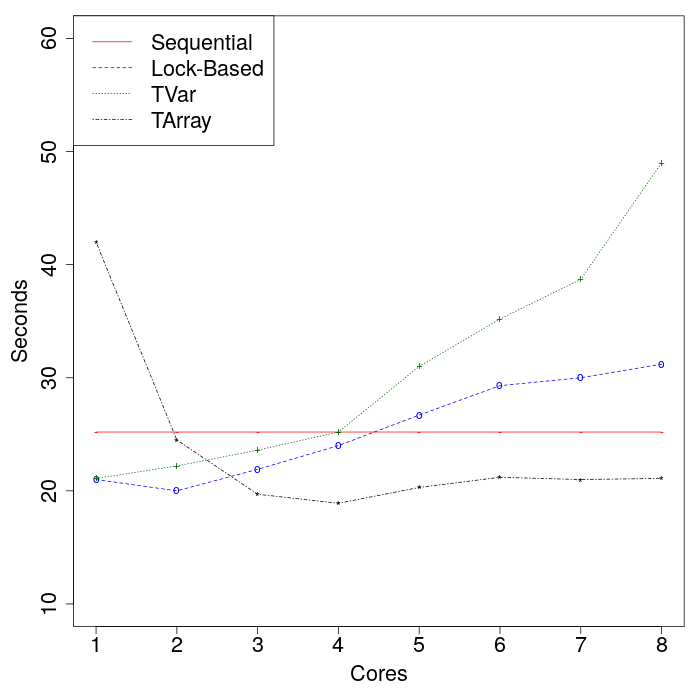
\includegraphics[width=0.6\textwidth, angle=0]{./fig/concurrentabs/sugarscape/sugarscape_varyingcores_constagents.png}
	\caption{Performance comparison of \textit{Sequential}, \textit{Lock-Based}, \textit{TVar} and \textit{TArray} Sugarscape implementations on varying cores with 50x50 environment and 500 initial agents.}
	\label{fig:sugarscape_varyingcores_constagents}
\end{figure}

\begin{table}
	\centering
  	\begin{tabular}{ c || c | c }
        Cores & TVar  & TArray  \\ \hline \hline 
    		1     & 0.00  & 0.00    \\ \hline
   		2     & 1.04  & 0.02    \\ \hline
   		3     & 2.15  & 0.04    \\ \hline
   		4     & 3.20  & 0.06    \\ \hline
   		5     & 4.06  & 0.07    \\ \hline
   		6     & 5.02  & 0.09    \\ \hline
   		7     & 6.09  & 0.10    \\ \hline
   		8     & 8.45  & 0.11    \\ \hline \hline
   	\end{tabular}
 
  	\caption{Retry ratio comparison (lower is better) of the \textit{TVar} and \textit{TArray} Sugarscape implementations under varying cores with 50x50 environment and 500 initial agents.}
	\label{tab:sugarscape_retry_ratios}
\end{table}

As expected, the \textit{Sequential} implementation is the slowest, with \textit{TArray} being the fastest except on 1 and 2 cores, where unexpectedly the \textit{Lock-Based} implementation performed best. Interestingly the \textit{TVar} implementation was the worst performing of the concurrent implementations.

The reason for the bad performance of \textit{TVar} is that using a \texttt{TVar} to share the environment is a very inefficient choice: \textit{every} write to a cell leads to a retry independent of whether the reading agent reads that changed cell or not, because the data structure cannot distinguish between individual cells. By using a \texttt{TArray}, we can avoid the situation where a write to a cell in a far distant location of the environment will lead to a retry of an agent which never even touched that cell. The inefficiency of \textit{TVar} is also reflected in the fact that the \textit{Lock-Based} implementation outperforms it on all cores. The sweet spot is at 3 cores in both cases, after which decreasing performance is the result. This is due to very similar approaches because both operate on the whole environment instead of only the cells as \textit{TArray} does. In case of the \textit{Lock-Based} approach, the lock contention increases, whereas in the \textit{TVar} approach, the retries start to dominate (see Table \ref{tab:sugarscape_retry_ratios}).

Interestingly, the performance of the \textit{TArray} implementation is the \textit{worst} amongst all on 1 core. We attribute this to the overhead incurred by STM, which dramatically adds up in terms of a sequential execution.

\subsection{Scaling Up Agents}
So far, we kept the initial number of agents at 500, which due to the model specification, quickly drops and stabilises around 200 due to the carrying capacity of the environment as described in the book \cite{epstein_growing_1996} section \textit{Carrying Capacity} (p. 30).

We now measure the performance of our approaches under an increased number of agents. For this we slightly change the implementation: when an agent dies it spawns a new one, which is inspired by the ageing and birthing feature of Chapter III in the book \cite{epstein_growing_1996}. This ensures that we keep the number of agents roughly constant (it still fluctuates but doesn't drop to low levels) over the whole duration. This ensures a constant load of concurrent agents interacting with each other and also demonstrates the ability to terminate and fork threads dynamically during the simulation.

Except for the \textit{Sequential} approach, we ran all experiments with 4 cores. We looked into the performance of 500, 1,000, 1,500, 2,000 and 2,500 (maximum possible capacity of the 50x50 environment). The results are reported in Table \ref{tab:sugarscape_varyingagents_constcores} and plotted in Figure \ref{fig:sugarscape_varyingagents_constcores}.

\begin{table}
	\centering
  	\begin{tabular}{ c || c | c | c | c }
        Agents  & Sequential    & Lock-Based    & TVar          & TArray                \\ \hline \hline 
    	    500     & 70.1 (0.41)   & 67.9 (0.13)   & 69.1 (0.34)   & \textbf{25.7} (0.42)  \\ \hline
   		1,000   & 145.0 (0.11)  & 130.0 (0.28)  & 136.0 (0.16)  & \textbf{38.8} (1.43)  \\ \hline
   		1,500   & 220.0 (0.14)  & 183.0 (0.83)  & 192.0 (0.73)  & \textbf{40.1} (0.25)  \\ \hline
   		2,000   & 213.0 (0.69)  & 181.0 (0.84)  & 214.0 (0.53)  & \textbf{49.9} (0.82)  \\ \hline
   		2,500   & 193.0 (0.16)  & 272.0 (0.81)  & 147.0 (0.32)  & \textbf{55.2} (1.04)  \\ \hline \hline
   	\end{tabular}
  	
  	\caption{Performance comparison of \textit{Sequential}, \textit{Lock-Based}, \textit{TVar} and \textit{TArray} Sugarscape implementations with varying agent numbers and 50x50 environment on 4 cores (except \textit{Sequential}). Timings in seconds (lower is better), standard deviation in parentheses.}
	\label{tab:sugarscape_varyingagents_constcores}
\end{table}

\begin{figure}
	\centering
	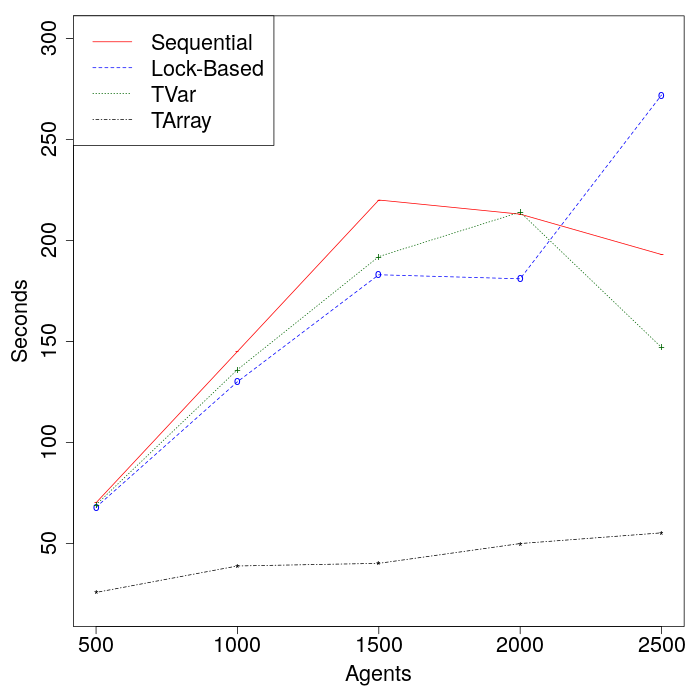
\includegraphics[width=0.6\textwidth, angle=0]{./fig/concurrentabs/sugarscape/sugarscape_varyingagents_constcores.png}
	\caption{Performance comparison of \textit{Sequential}, \textit{Lock-Based}, \textit{TVar} and \textit{TArray} Sugarscape implementations with varying agent numbers and 50x50 environment on 4 cores (except \textit{Sequential}).}
	\label{fig:sugarscape_varyingagents_constcores}
\end{figure}

As expected, the \textit{TArray} implementation outperforms all others substantially and scales up much smoothly. Also, \textit{Lock-Based} performs better than the \textit{TVar}.

What seems to be very surprising is that in the \textit{Sequential} and \textit{TVar} cases the performance with 2,500 agents is \textit{better} than the one with 2,000 agents. The reason for this is that in the case of 2,500 agents, an agent can't move anywhere because all cells are already occupied. In this case the agent will not rank the cells in order of their payoff (max sugar) as to where to move, but just stays where it is. We hypothesize that due to Haskell's laziness the agents never actually look at the content of the cells, but only the number, which means that the cells themselves are never evaluated and this further increases performance. This leads to the better performance in case of \textit{Sequential} and \textit{TVar} because both exploit laziness. 
In the case of the \textit{Lock-Based} approach we still arrive at a lower performance level because the limiting factor is the unconditional locks. In the case of the \textit{TArray} approach we also arrive at a lower performance because it seems that STM perform reads on the neighbouring cells which are not subject to lazy evaluation.

In case of the \textit{Sequential} implementation with 2,000 agents we also arrive at a better performance than with 1,500, due to less space of the agents for free movement, exploiting laziness as in the case with 2,500 agents. In the case of the \textit{Lock-Based} approach we see similar behaviour, where the performance with 2,000 agents is better than with 1,500. It is not quite clear why this is the case, given the dramatically \textit{lower} performance with 2,500 agents but it seems that 2,000 agents create much less lock contention due to lower free space, whereas 2,500 agents create a lot more lock contention due to no free space available at all.

We also measured the average retries both for \textit{TVar} and \textit{TArray} under 2,500 agents where the \textit{TArray} approach shows best scaling performance with 0.01 retries whereas \textit{TVar} averages at 3.28 retries. Again, this can be attributed to the better transactional data structure which reduces the retry ratio substantially to near-zero levels.

\subsection{Going Large Scale}
To test how far we can scale up the number of cores in the \textit{TArray} case, we ran the two experiments, carrying capacity (500 agents) and rebirthing (2500 agents), on an Amazon EC \texttt{m5ad.16xlarge} instance with 16, 32 and 64 cores to see if we run into decreasing returns. The results are reported in Table \ref{tab:sug_varying_cores_amazon}.

\begin{table}
	\centering	
 
  	\begin{tabular}{ c || c | c }
        Cores  & Carrying Capacity  & Rebirthing    \\ \hline \hline 
    	    16     & 11.9 (0.21)        & 46.6 (0.07)   \\ \hline
   		32     & 12.8 (0.29)        & 76.4 (0.01)   \\ \hline
   		64     & 14.6 (0.09)        & 99.1 (0.01)   \\ \hline \hline
   	\end{tabular}

  	\caption{Sugarscape \textit{TArray} performance on 16, 32 and 64 cores an Amazon EC \texttt{m5ad.16xlarge} instance. Timings in seconds (lower is better). Retry ratios in parentheses.}
	\label{tab:sug_varying_cores_amazon}
\end{table}

Unlike in the SIR model, Sugarscapes STM \textit{TArray} implementation does not scale up beyond 16 cores. We attribute this to a mix of retries and Amdahl's law. As retries are much more expensive in the case of Sugarscape compared to SIR, even a small increase in the retry ratio (see Table \ref{tab:sugarscape_retry_ratios}), leads to reduced performance. On the other hand, although the retry ratio decreases as the number of cores increases, the ratio of parallelisable work diminishes and we get bound by the sequential part of the program.

\subsection{Comparison with Other Approaches}
The paper \cite{lysenko_framework_2008} reports a performance of 2,000 steps per second on a GPU on a 128x128 grid. Our best performing implementation, \textit{TArray} with 500 rebirthing agents, arrives at a performance of 39 steps per second and is therefore clearly slower. However, the very high performance on the GPU does not concern us here as it follows a very different approach than ours. We focus on speeding up implementations on the CPU as directly as possible without locking overhead. When following a GPU approach, one needs to map the model to the GPU which is a delicate and non-trivial matter. With our approach we show that speed up with concurrency is very possible without the low-level locking details or the need to map to GPU. Additionally, some features like bilateral trading between agents, where a pair of agents needs to come to a conclusion over multiple synchronous steps, is difficult to implement on a GPU whereas this should be not as hard using STM.

Note that we kept the grid size constant because we implemented the environment as a single agent which works sequentially on the cells to regrow the sugar. Obviously, this doesn't really scale up on parallel hardware and experiments, which we haven't included here due to lack of space. They show that the performance goes down dramatically when we increase the environment to 128x128 with same number of agents. This is the result of Amdahl's law, where the environment becomes the limiting \textit{sequential} factor of the simulation. Depending on the underlying data structure used for the environment, we have two options to solve this problem. In the case of the \textit{Sequential} and \textit{TVar} implementation we build on an indexed array, which can be updated in parallel using the existing data-parallel support in Haskell. In the case of the \textit{TArray} approach, we have no option but to run the update of every cell within its own thread. We leave both for further research as it is beyond the scope of this thesis.

\subsection{Summary}
This case study showed clearly that besides being substantially faster than the \textit{Sequential} implementation, an \textit{STM} implementation with the right transactional data structure is also able to perform considerably better than a \textit{Lock-Based} approach. This is true even in the case of the Sugarscape model, which has a much higher complexity in terms of agent behaviour and a dramatically increased number of writes to the environment.

Furthermore, this case study demonstrated that the selection of the right transactional data structure is of fundamental importance when using STM. Selecting the right transactional data structure is highly model-specific and can lead to dramatically different performance results. In this case study, the \textit{TArray} performed best due to many writes but in the SIR case study a \textit{TVar} showed good enough results due to the very low number of writes. When not carefully selecting the right transactional data structure, which supports fine-grained concurrency, a lock-based implementation might perform as well or even outperform the STM approach as can be seen when using the \texttt{TVar}.

Although the \texttt{TArray} is the better transactional data structure overall, it might come with an overhead, performing worse on low number of cores than a \textit{TVar}, \textit{Lock-Based} or even \textit{Sequential} approach, as seen with \textit{TArray} on 1 core. However, it has the benefit of quickly scaling up to multiple cores. Depending on the transactional data structure, scaling up to multiple cores hits a limit at some point. In the case of the \texttt{TVar} the best performance is reached with 3 cores. With the \texttt{TArray} we reached this limit around 16 cores.

The comparison between the \textit{Lock-Based} approach and the \textit{TArray} implementation seems to be a bit unfair due to a very different locking structure. A more suitable comparison would be to use an indexed Array with a tuple of \texttt{(MVar, IORef)}, holding a synchronisation primitive and reference for each cell to support fine-grained locking on the cell level. This would seem to be a more just comparison to the \textit{TArray} where fine-grained transactions happen on the cell level. However, due to the model semantics, this approach is actually not possible. As already expressed in the experiment's description, in Sugarscape an agent needs a consistent view of the whole environment for the whole duration of an agent execution due to the fact that agents don't only write their own locations but change also other locations. If we used an indexed array we would also run into data races because the agents need to hold all relevant cells. The cells can't be grabbed in one atomic instruction, but only one after another, which makes it highly susceptible to data races. Therefore, we could run into deadlocks if two agents are acquiring locks because they are taken after another and therefore subject to races where they end up holding a lock the other needs.